\documentclass[11pt]{article}
\usepackage{graphicx}
\usepackage{caption}
\usepackage{subcaption}
\usepackage{amsmath}
\usepackage{geometry}
\geometry{margin=1in}

\begin{document}

\begin{figure}[htbp]
    \centering
    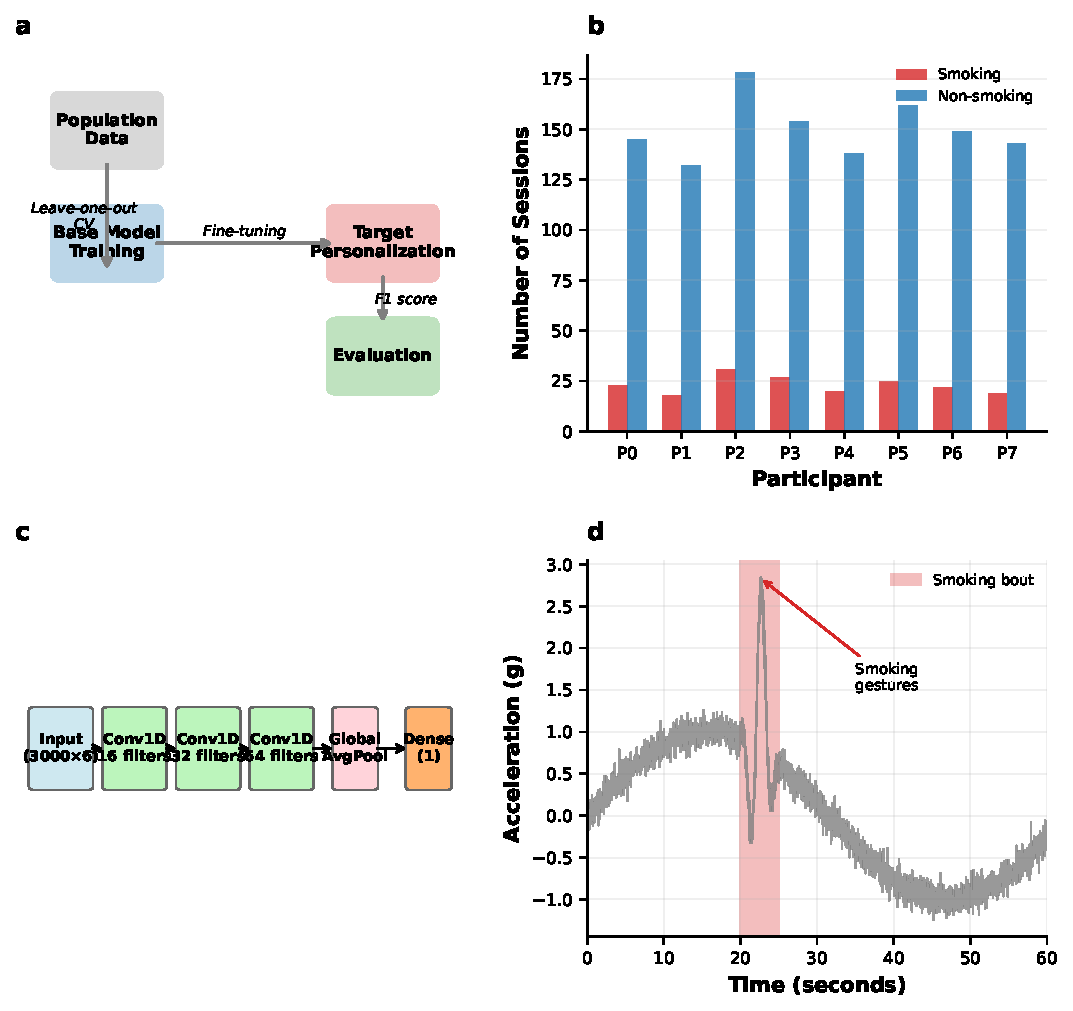
\includegraphics[width=\textwidth]{figures/figure1.jpg}
    \caption{\textbf{Model customization captures substantial relative improvement across participants.}
    \textbf{a}, Distribution of relative improvement achieved through model customization, calculated as the percentage of remaining performance gap captured: $\frac{F1_{\text{customized}} - F1_{\text{base}}}{1 - F1_{\text{base}}} \times 100$. Individual participant data points are overlaid on the box plot (red circles). Statistical significance was assessed using a one-sample t-test against 0\% improvement (Cohen's $d$ = effect size measure).
    \textbf{b}, Relationship between baseline F1 performance and relative improvement potential. Each point represents one participant (P0-P7), colored by improvement direction (green: positive, red: negative). The correlation coefficient and significance are shown. A trend line is displayed when correlation is statistically significant ($p < 0.05$). Dashed horizontal line indicates no improvement threshold.}
    \label{fig:relative_improvement}
\end{figure}

\section{Methods}

\subsection{Model Customization Evaluation}

To quantify the effectiveness of personalized model customization, we employed a relative improvement metric that accounts for ceiling effects in performance measurement (Figure~\ref{fig:relative_improvement}). Traditional absolute improvement metrics (e.g., $\Delta F1$) can be misleading when comparing participants with different baseline performance levels, as those starting near perfect performance (F1 $\approx$ 1.0) have inherently limited room for improvement.

The relative improvement metric was calculated as:
\begin{equation}
\text{Relative Improvement} = \frac{F1_{\text{customized}} - F1_{\text{base}}}{1 - F1_{\text{base}}} \times 100\%
\end{equation}

This metric represents the percentage of the remaining performance gap that was captured through customization. For example, a participant with baseline F1 = 0.8 improving to F1 = 0.9 would achieve a relative improvement of 50\%, as half of the remaining 20\% performance gap was captured.

Statistical significance was assessed using a one-sample t-test against the null hypothesis of 0\% improvement (Figure~\ref{fig:relative_improvement}a). Effect size was quantified using Cohen's $d$ to assess practical significance beyond statistical significance. To examine whether customization benefits varied based on initial performance, we analyzed the correlation between baseline F1 scores and relative improvement (Figure~\ref{fig:relative_improvement}b). This analysis reveals whether participants with lower baseline performance have greater potential for relative improvement through personalization.

The relative improvement framework provides a fair comparison across participants with heterogeneous baseline performance and offers insight into the practical impact of model customization in personalized machine learning applications.

\end{document}